\documentclass{article}
\usepackage[a4paper,left=3cm,right=3cm,top=3cm,bottom=3cm]{geometry}
\usepackage[utf8]{inputenc}
\usepackage[T1]{fontenc}
\usepackage{latexsym,amsfonts,amsmath,amssymb,amstext,graphicx,titlesec,ae,aecompl,mathtools,tabularx, multirow, cancel, nicefrac,subcaption, blindtext, floatrow}
\setlength{\parindent}{0pt}
\newfloatcommand{capbtabbox}{table}[][\FBwidth]


\begin{document}

\begin{titlepage}
       \begin{center}
             \begin{huge}
				   %% Update assignment number here
                   \textbf{Assignment 2}
             \end{huge}
       \end{center}

       \begin{center}
             \begin{large}
                   Computational Intelligence, SS2020
             \end{large}
       \end{center}

       \begin{center}
 \begin{tabularx}{\textwidth}{|>{\hsize=.33\hsize}X|>{\hsize=.33\hsize}X|>{\hsize=.33\hsize}X|} 

                   \hline
                   \multicolumn{3}{|c|}{\textbf{Team Members}} \\
                   \hline
                   Last name & First name & Matriculation Number \\
                   \hline
                   Blöcher & Christian & 01573246 \\
                   \hline
                   Bürgener & Max & 01531577 \\
                   \hline
                    &  &  \\
                   \hline

             \end{tabularx}
       \end{center}
\end{titlepage}

\section{Linear regression}

\subsection{Derivation of Regularized Linear Regression}

%\begin{itemize}

%    \begin{figure}[h]
%        \centering
%        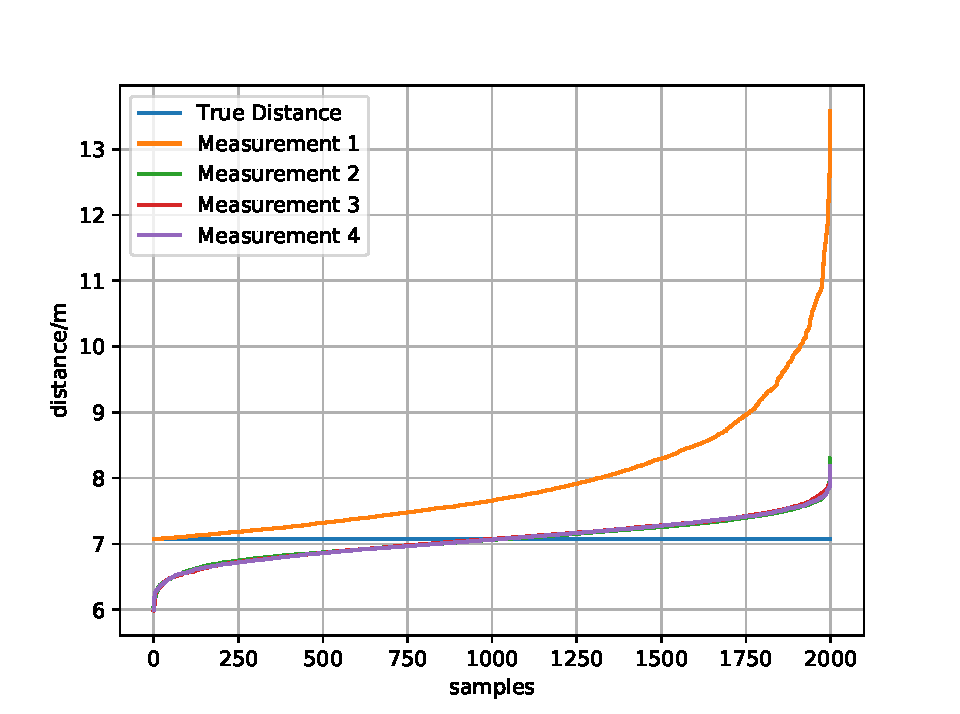
\includegraphics[width=\textwidth]{./Figures/scenario2_findexponential.pdf}
%        \caption{Scenario 2 with mixed measurement models for the anchors}
%        \label{fig:scenario2_findexponential}
%    \end{figure}
    
%    \item In figure \ref{fig:scenario2_findexponential} we can see that in scenario 2 the distance measurements from anchor 1 is exponentially distributed. It is the only distribution which is bigger than the true distance for all samples and its slope is rising exponentially for rising x-values.
    
%\end{itemize}

\subsection{Linear Regression with polynomial features}


\begin{figure}[!ht]
\centering
\makebox[\textwidth]{
\begin{subfigure}{0.65\textwidth}
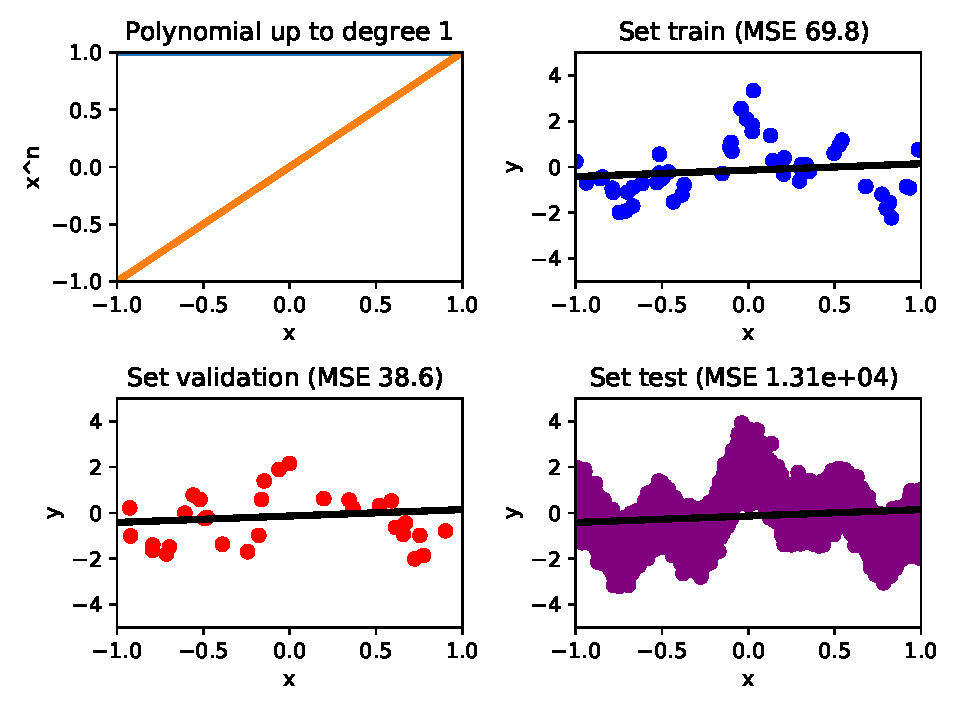
\includegraphics[width=\textwidth]{./Figures/linreg_poly1_deg1.pdf}
\caption{$n=1$}
\end{subfigure}
\begin{subfigure}{0.65\textwidth}
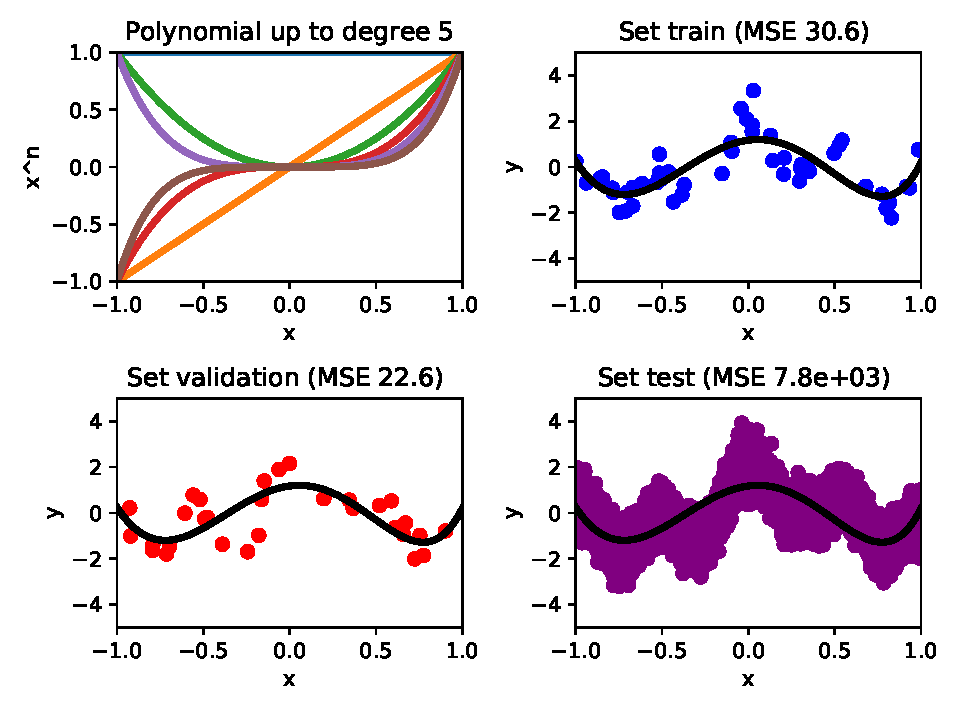
\includegraphics[width=\textwidth]{./Figures/linreg_poly1_deg5.pdf}
\caption{$n=5$}
\end{subfigure}
}

\makebox[\textwidth]{
\begin{subfigure}{0.65\textwidth}
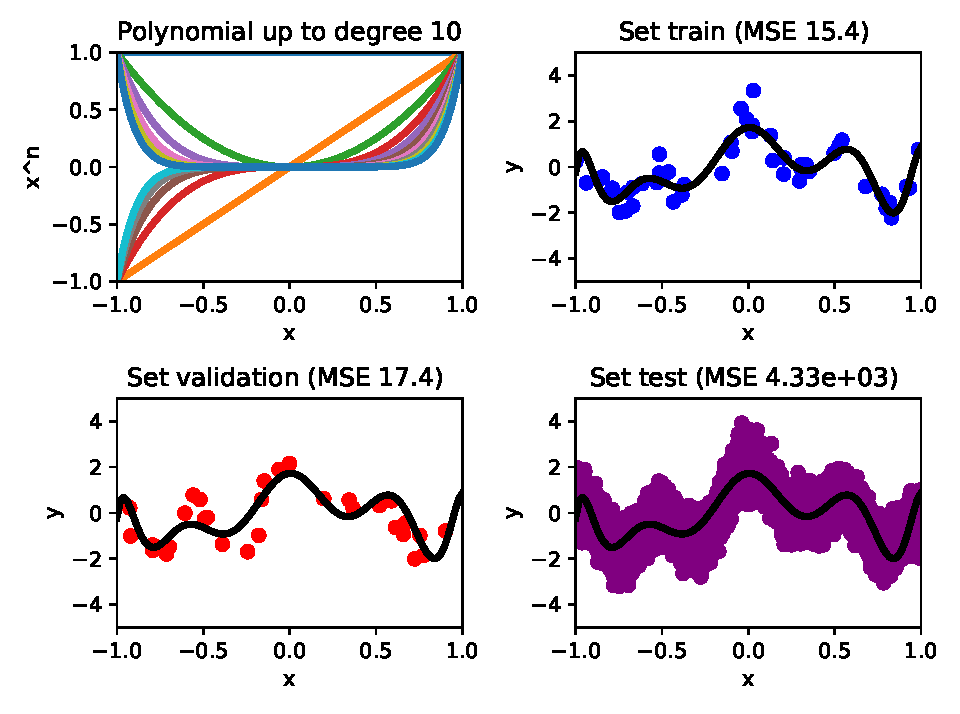
\includegraphics[width=\textwidth]{./Figures/linreg_poly1_deg10.pdf}
\caption{$n=10$}
\end{subfigure}
\begin{subfigure}{0.65\textwidth}
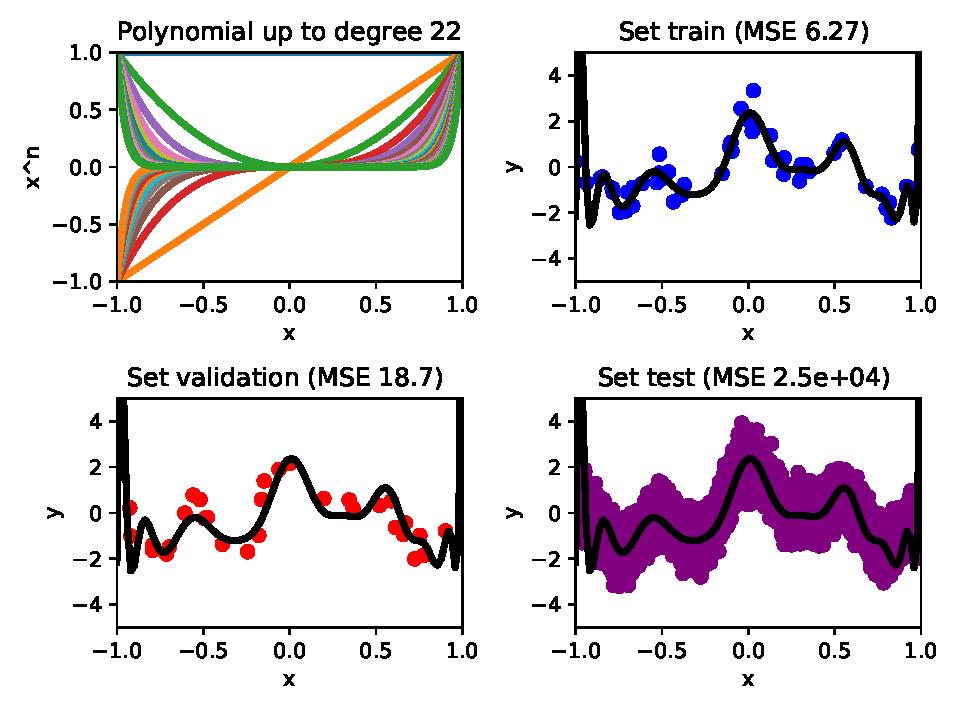
\includegraphics[width=\textwidth]{./Figures/linreg_poly1_deg22.pdf}
\caption{$n=22$}
\end{subfigure}
}
\caption{Results of Linear Regression for varying polynomial degree $n$.}
\label{linreg_poly1}
\end{figure}

\begin{figure}[!ht]
\makebox[\textwidth]{
\begin{subfigure}{0.65\textwidth}
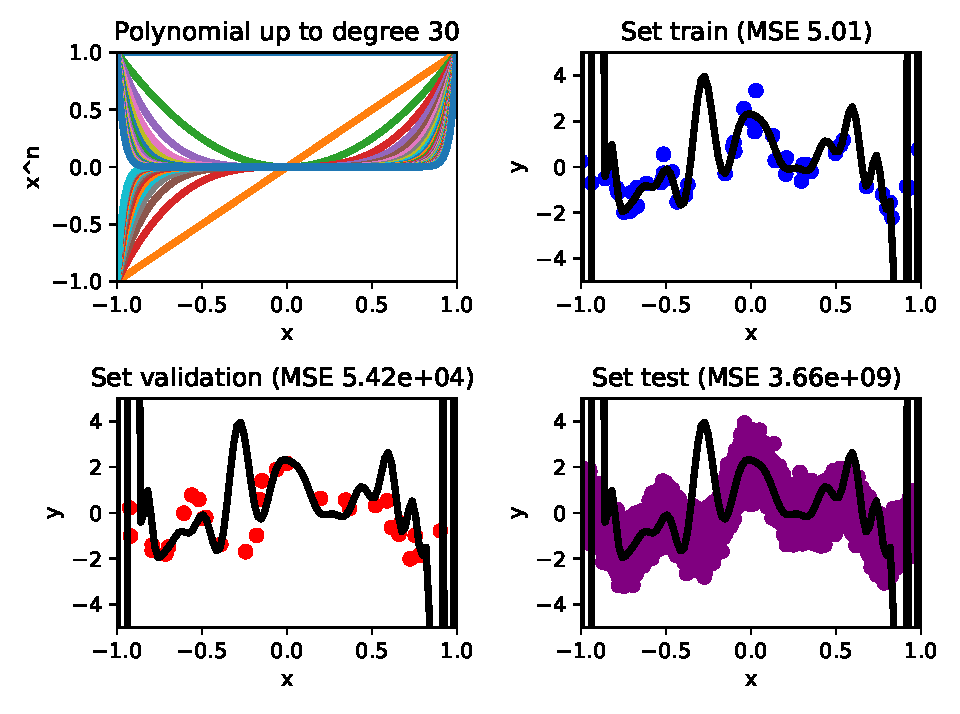
\includegraphics[width=\textwidth]{./Figures/linreg_poly2_besttrain.pdf}
\caption{Training set, $n=30$}
\end{subfigure}
\begin{subfigure}{0.65\textwidth}
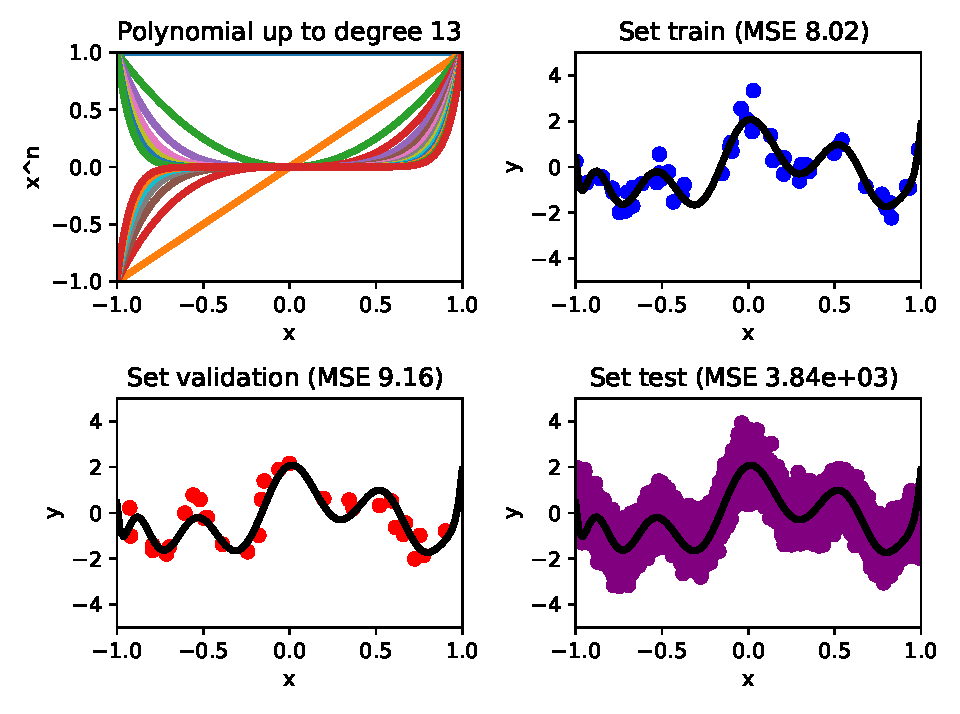
\includegraphics[width=\textwidth]{./Figures/linreg_poly3_bestval.pdf}
\caption{Validation set, $n=13$}
\end{subfigure}
}
\caption{Results with lowest cost on training and validation set.}
\label{linreg_poly23}
\end{figure}

\begin{figure}[!ht]
\centering
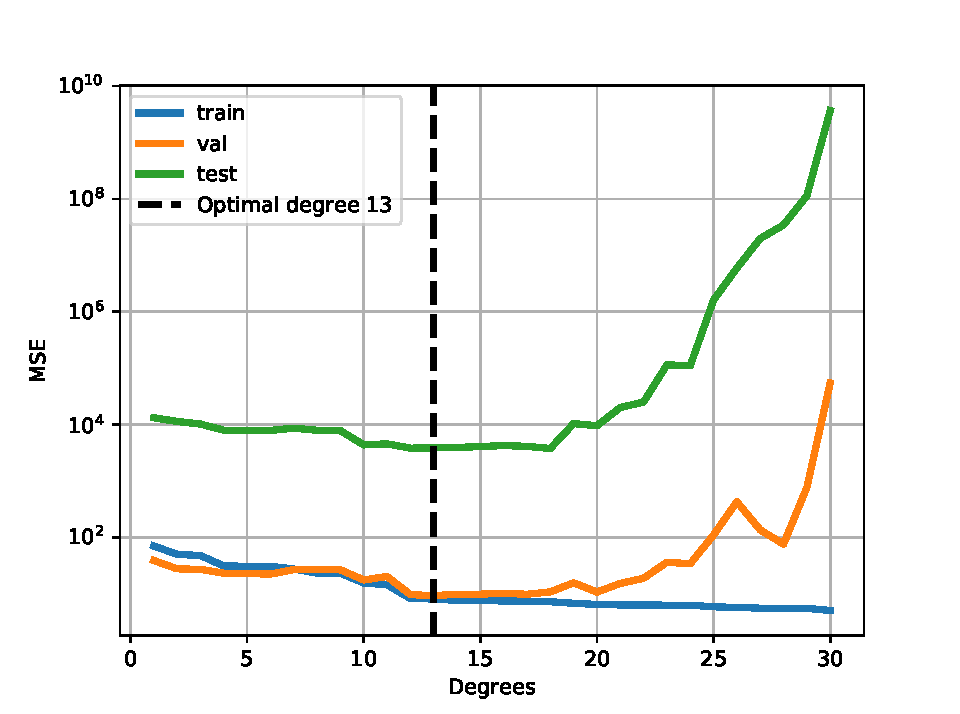
\includegraphics[width=0.8\textwidth]{./Figures/linreg_poly4_errors.pdf}
\caption{Training, validation and testing costs as a function of the polynomial degree $n$.}
\label{linreg_poly4}
\end{figure}


\subsection{(Bonus) Linear Regression with radial basis functions}

\begin{figure}[!ht]
\centering
\makebox[\textwidth]{
\begin{subfigure}{0.65\textwidth}
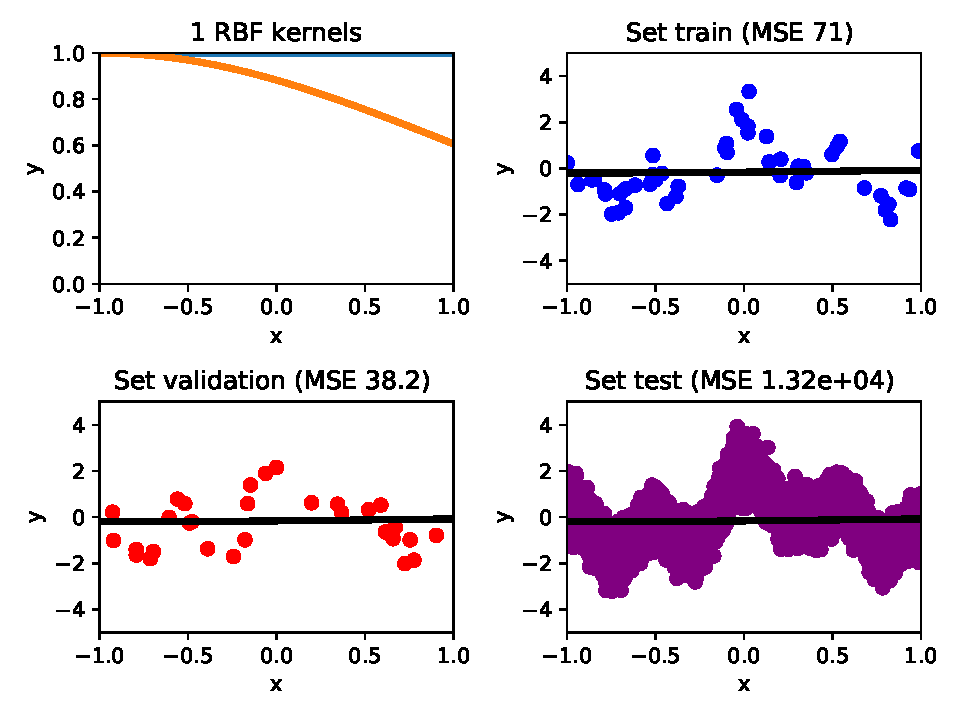
\includegraphics[width=\textwidth]{./Figures/linreg_rbf1_ncent1.pdf}
\caption{$l=1$}
\end{subfigure}
\begin{subfigure}{0.65\textwidth}
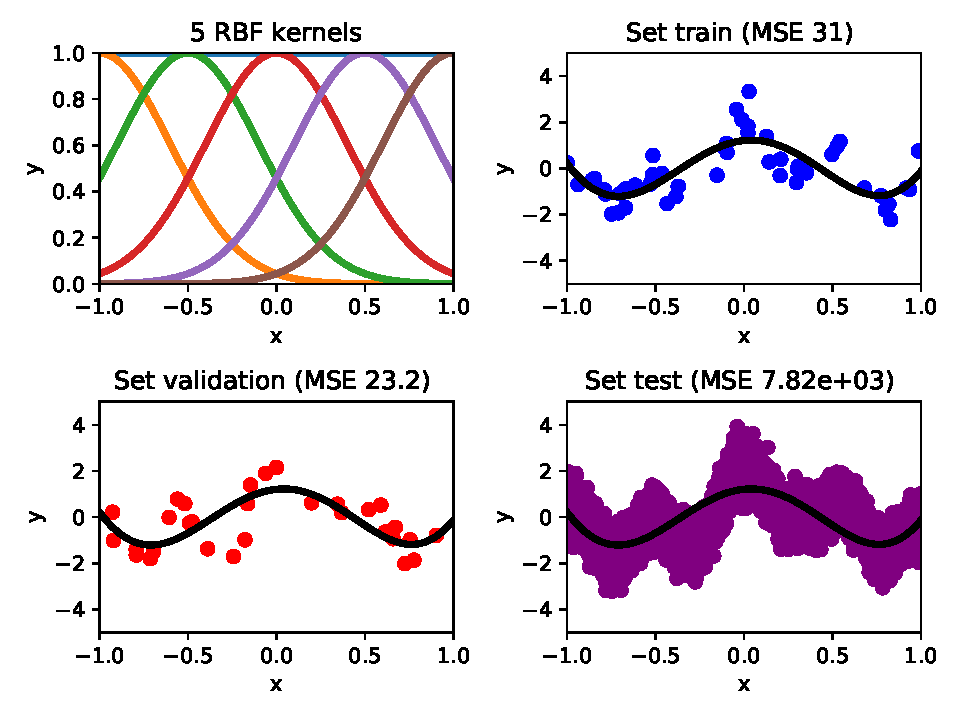
\includegraphics[width=\textwidth]{./Figures/linreg_rbf1_ncent5.pdf}
\caption{$l=5$}
\end{subfigure}
}

\makebox[\textwidth]{
\begin{subfigure}{0.65\textwidth}
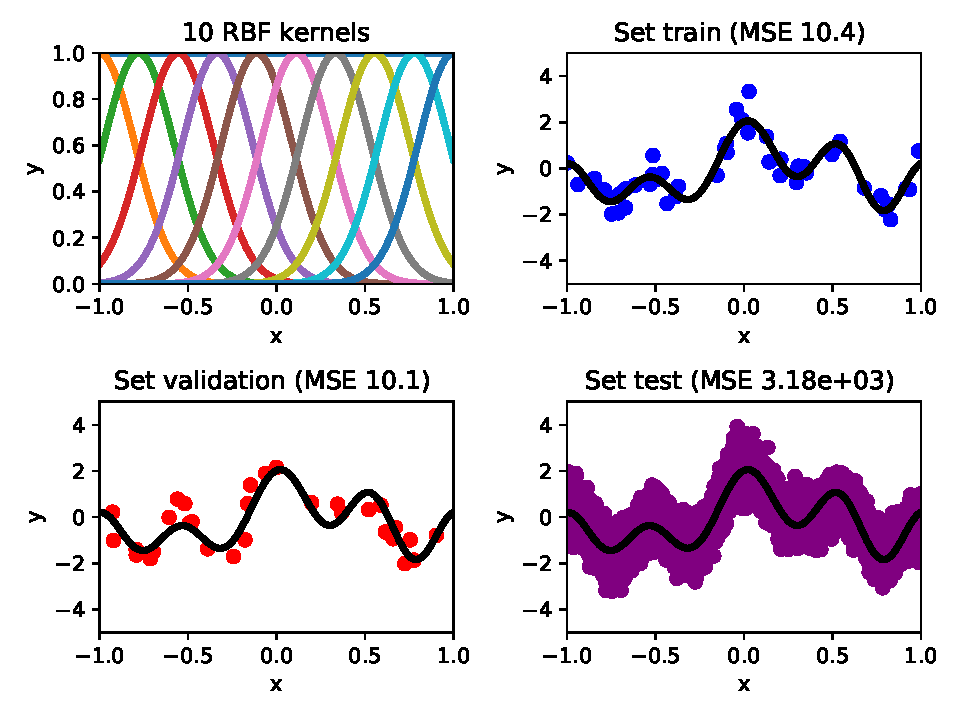
\includegraphics[width=\textwidth]{./Figures/linreg_rbf1_ncent10.pdf}
\caption{$l=10$}
\end{subfigure}
\begin{subfigure}{0.65\textwidth}
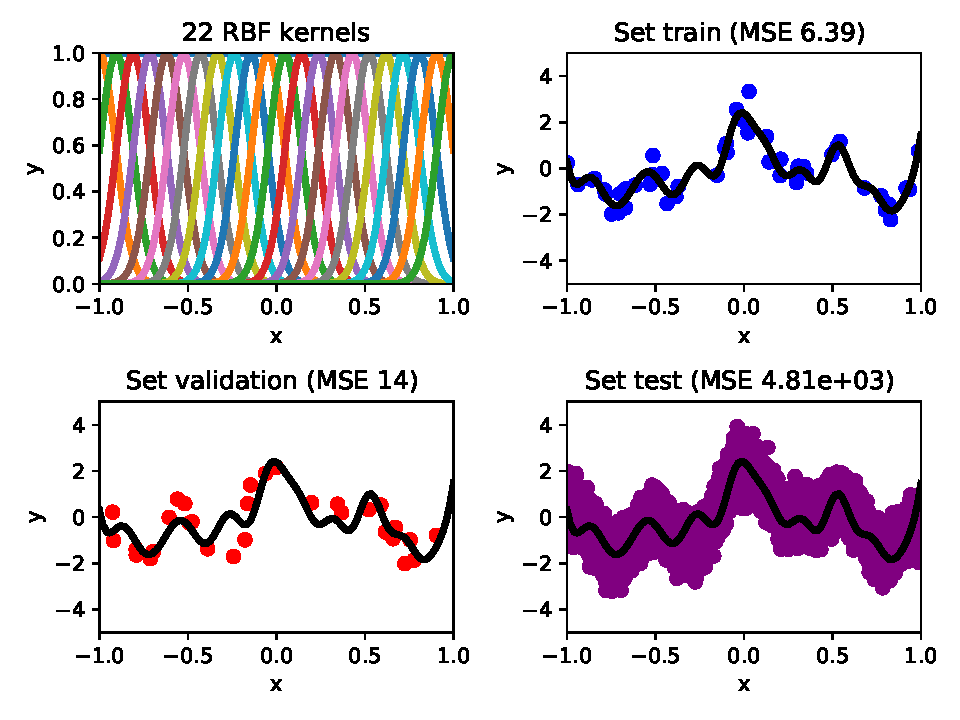
\includegraphics[width=\textwidth]{./Figures/linreg_rbf1_ncent22.pdf}
\caption{$l=22$}
\end{subfigure}
}
\caption{Results of Linear Regression for varying degree $l$.}
\label{linreg_rbf1}
\end{figure}

\begin{figure}[!ht]
\makebox[\textwidth]{
\begin{subfigure}{0.65\textwidth}
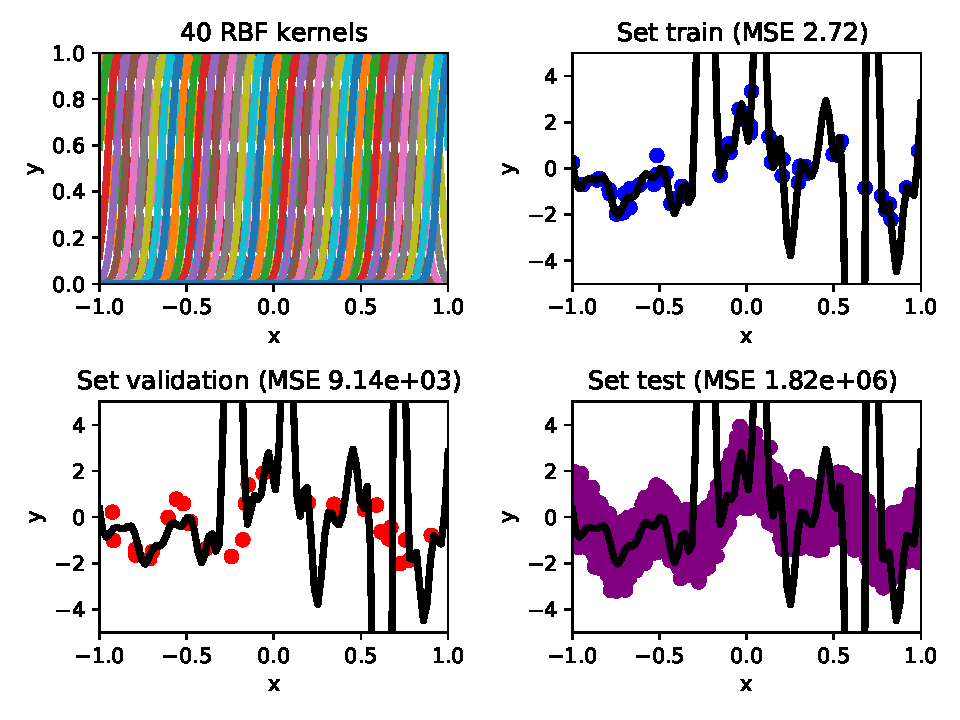
\includegraphics[width=\textwidth]{./Figures/linreg_rbf2_besttrain.pdf}
\caption{Training set, $l=40$}
\end{subfigure}
\begin{subfigure}{0.65\textwidth}
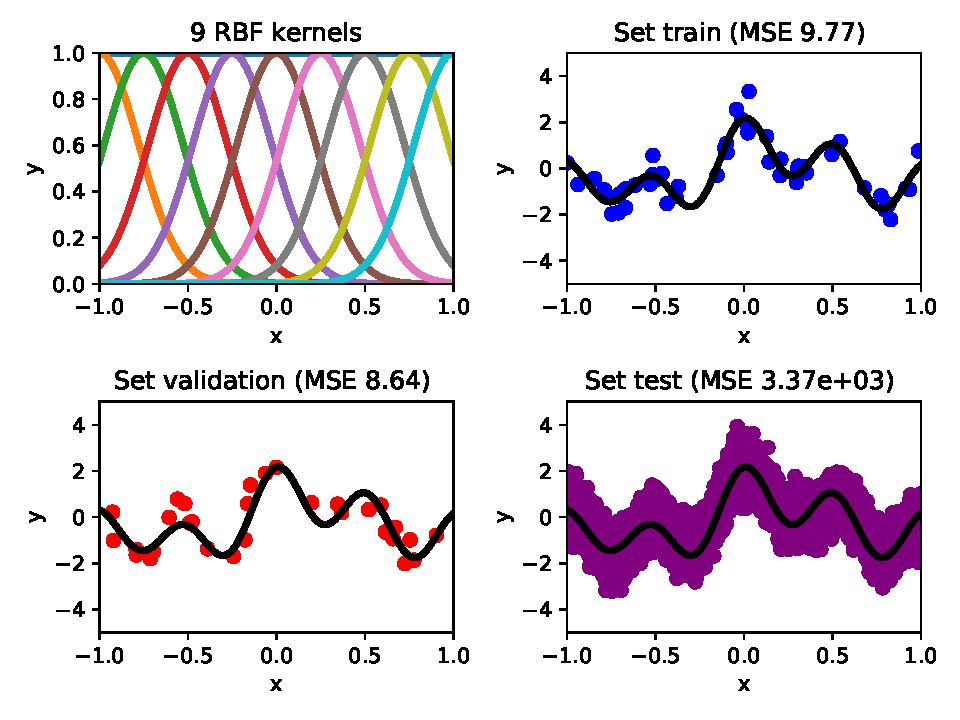
\includegraphics[width=\textwidth]{./Figures/linreg_rbf3_bestval.pdf}
\caption{Validation set, $l=9$}
\end{subfigure}
}
\caption{Results with lowest cost for training and validation set.}
\label{linreg_rbf23}
\end{figure}

\begin{figure}[!ht]
\centering
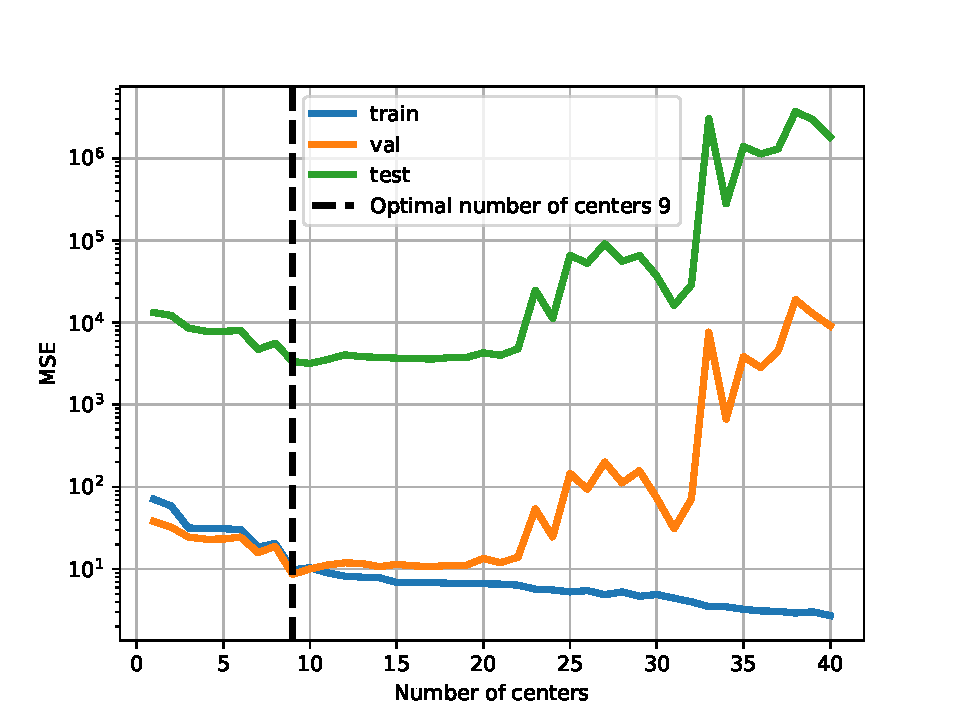
\includegraphics[width=0.8\textwidth]{./Figures/linreg_rbf4_errors.pdf}
\caption{Training, validation and testing costs as a function of the degree $l$.}
\label{linreg_rbf4}
\end{figure}


\section{Logistic Regression}
\subsection{Derivation of Gradient}


\subsection{Logistic Regression training with gradient descent}

\begin{figure}[!ht]
\centering
\makebox[\textwidth]{
\begin{subfigure}{0.5\textwidth}
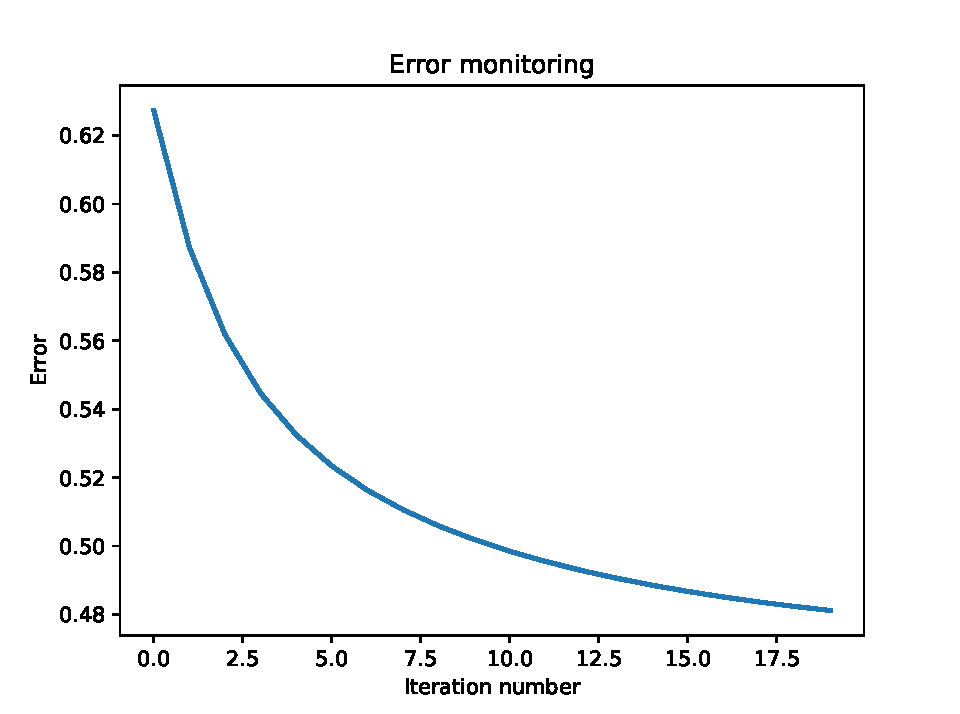
\includegraphics[width=\textwidth]{./Figures/logreg2_iter20_error.pdf}
\caption{Error, 20 iterations}
\end{subfigure}
\begin{subfigure}{0.5\textwidth}
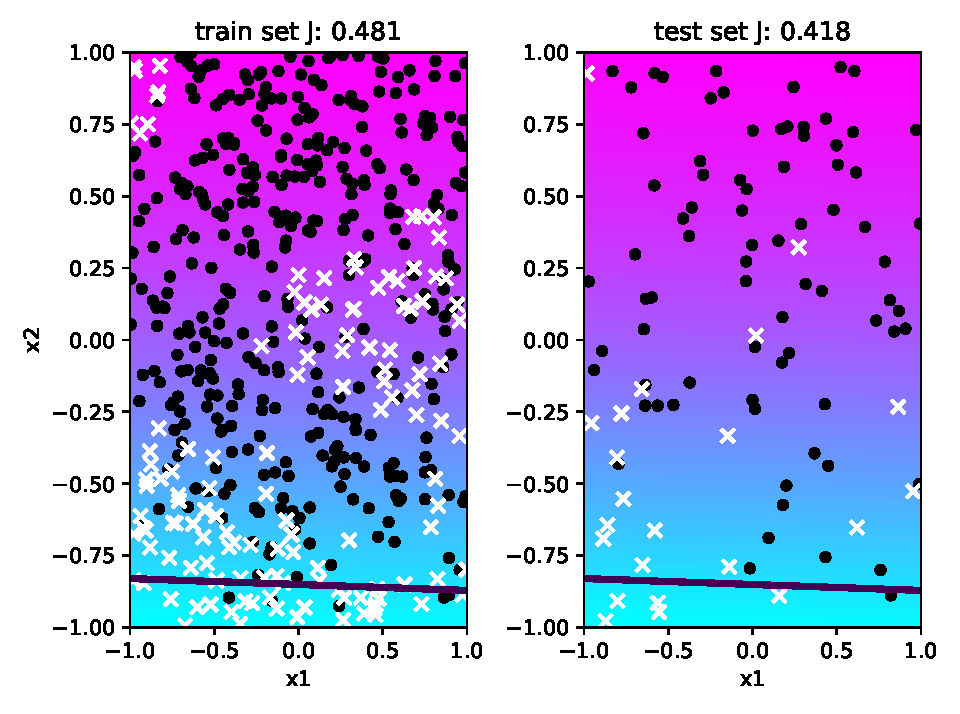
\includegraphics[width=\textwidth]{./Figures/logreg2_iter20_decbound.pdf}
\caption{Decision boundary, 20 iterations}
\end{subfigure}
}

\makebox[\textwidth]{
\begin{subfigure}{0.5\textwidth}
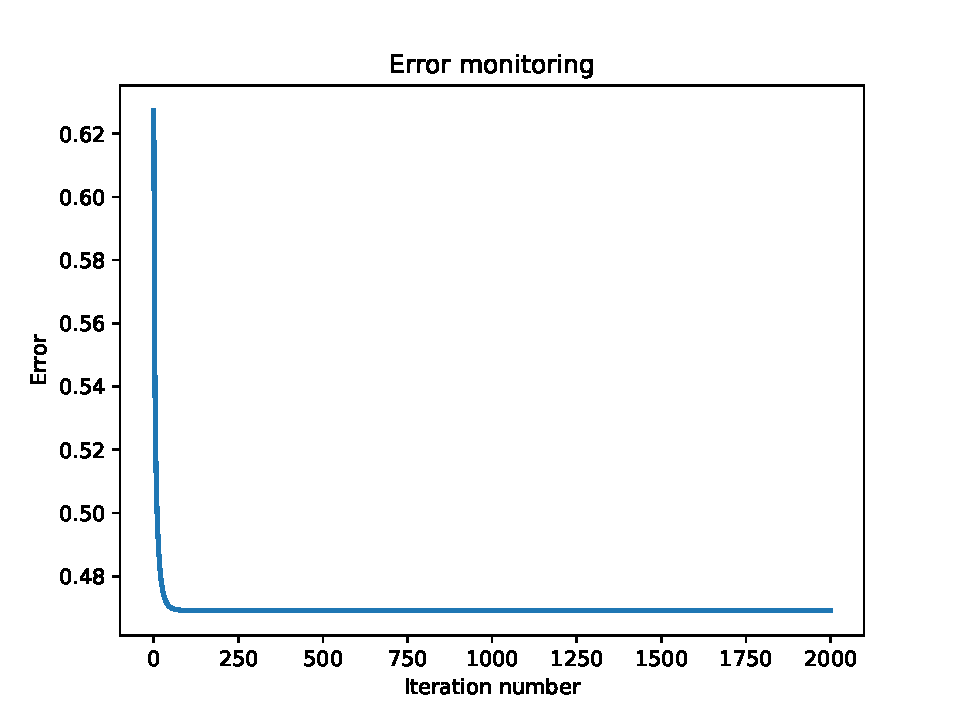
\includegraphics[width=\textwidth]{./Figures/logreg2_iter2000_error.pdf}
\caption{Error, 2000 iterations}
\end{subfigure}
\begin{subfigure}{0.5\textwidth}
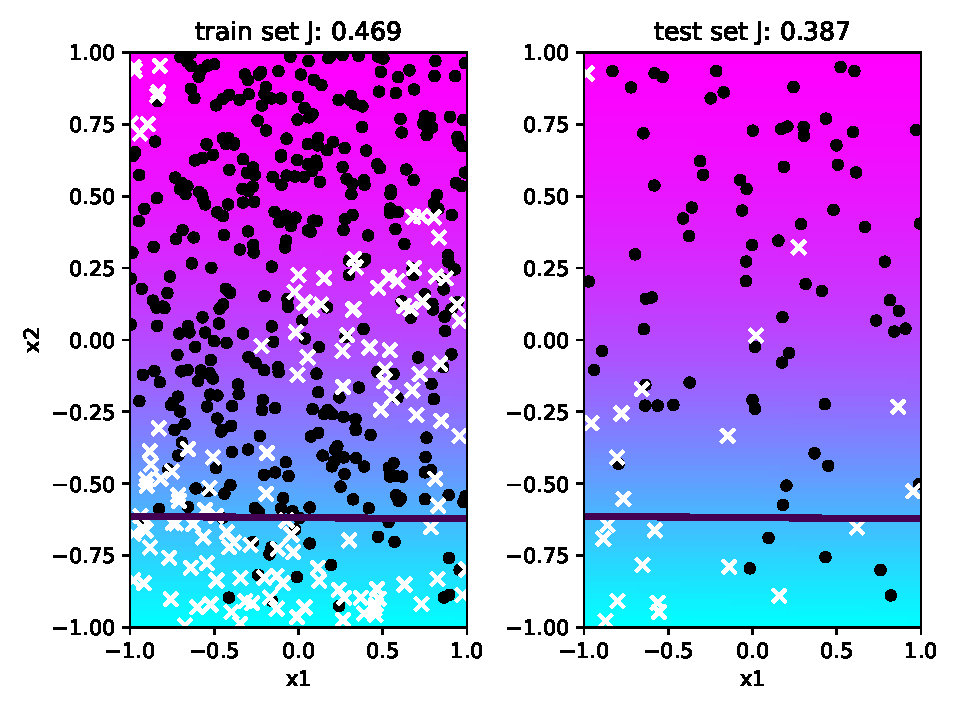
\includegraphics[width=\textwidth]{./Figures/logreg2_iter2000_decbound.pdf}
\caption{Decision boundary, 2000 iterations}
\end{subfigure}
}
\caption{GD errors and decision boundaries for varying number of iterations, degree $l=1$ and learning rate $\eta=1$.}
\label{logreg2}
\end{figure}

\begin{figure}[!ht]
\centering
\makebox[\textwidth]{
\begin{subfigure}{0.5\textwidth}
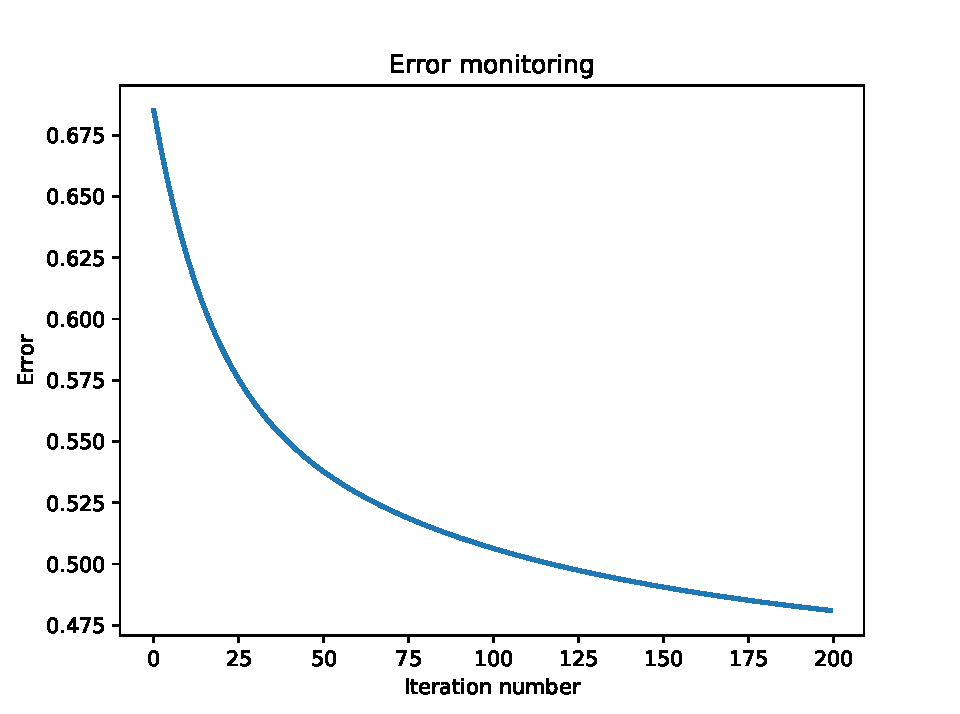
\includegraphics[width=\textwidth]{./Figures/logreg3_eta01_error.pdf}
\caption{Error, $\eta=0.1$}
\end{subfigure}
\begin{subfigure}{0.5\textwidth}
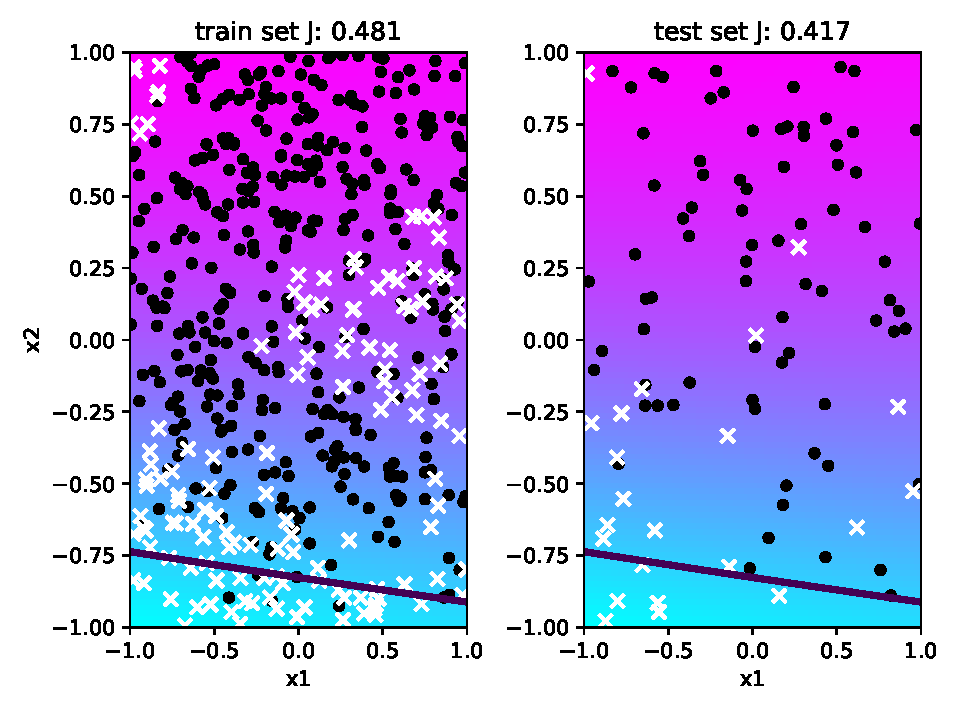
\includegraphics[width=\textwidth]{./Figures/logreg3_eta01_decbound.pdf}
\caption{Decision boundary, $\eta=0.1$}
\end{subfigure}
}

\makebox[\textwidth]{
\begin{subfigure}{0.5\textwidth}
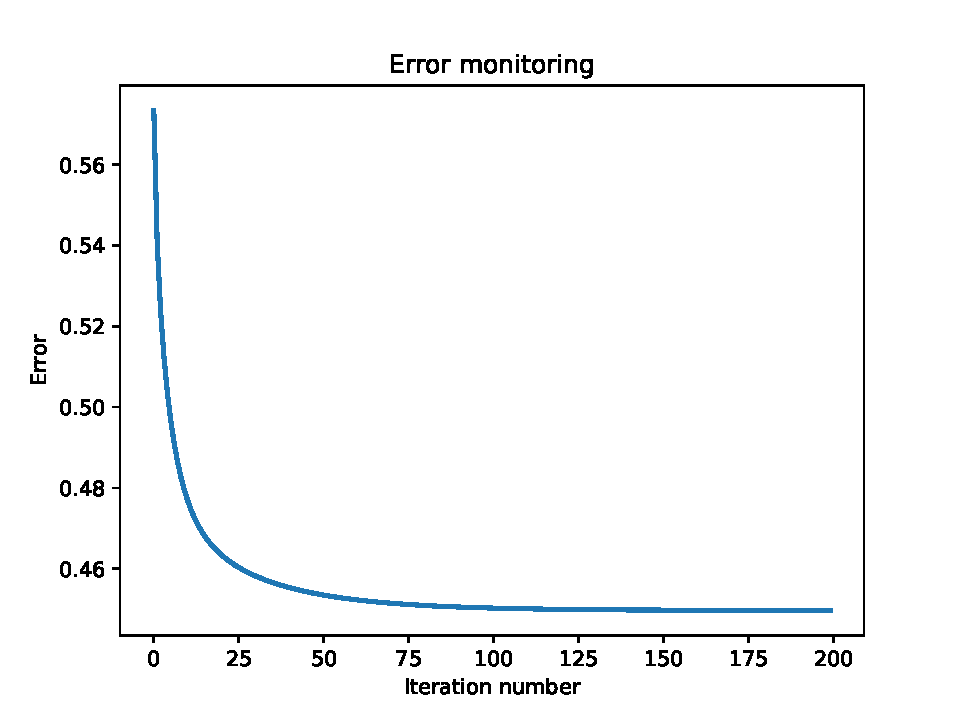
\includegraphics[width=\textwidth]{./Figures/logreg3_eta2_error.pdf}
\caption{Error, $\eta=2$}
\end{subfigure}
\begin{subfigure}{0.5\textwidth}
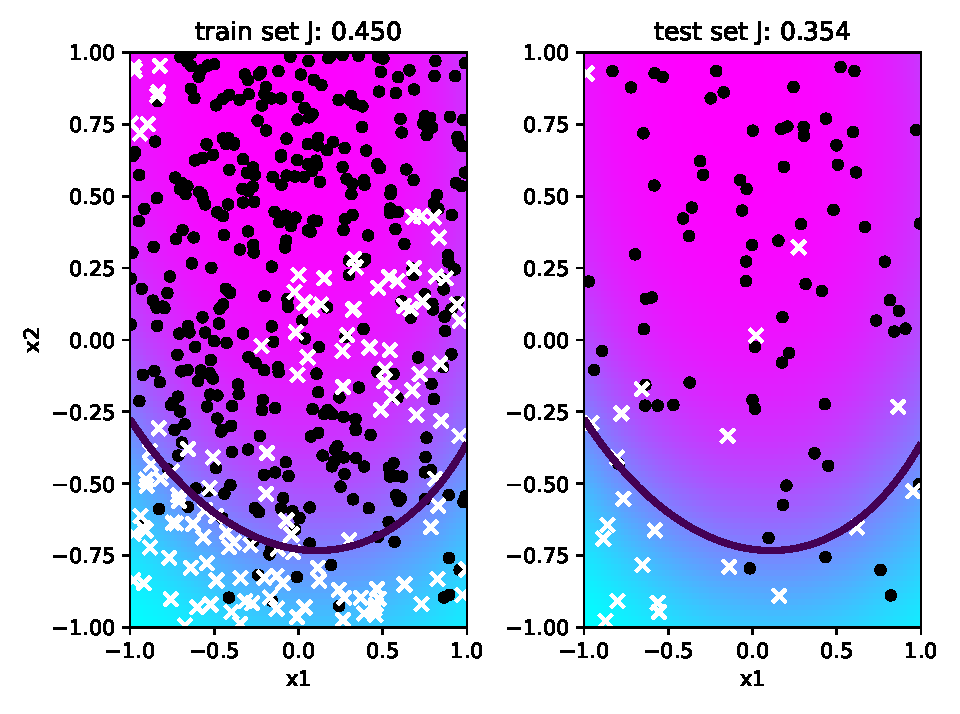
\includegraphics[width=\textwidth]{./Figures/logreg3_eta2_decbound.pdf}
\caption{Decision boundary, $\eta=2$}
\end{subfigure}
}

\makebox[\textwidth]{
\begin{subfigure}{0.5\textwidth}
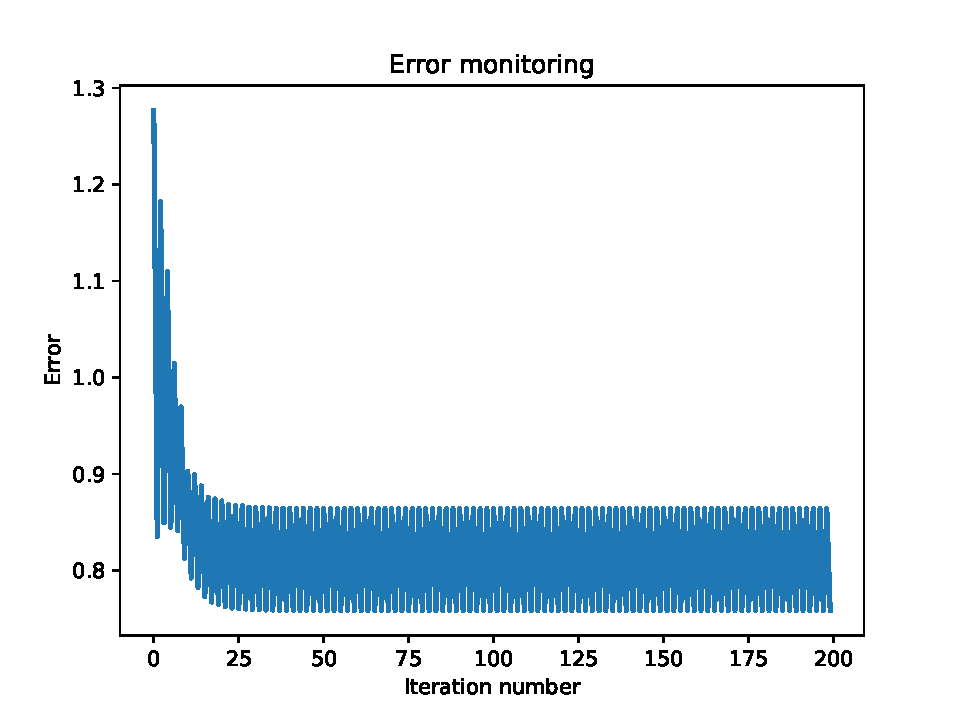
\includegraphics[width=\textwidth]{./Figures/logreg3_eta20_error.pdf}
\caption{Error, $\eta=20$}
\end{subfigure}
\begin{subfigure}{0.5\textwidth}
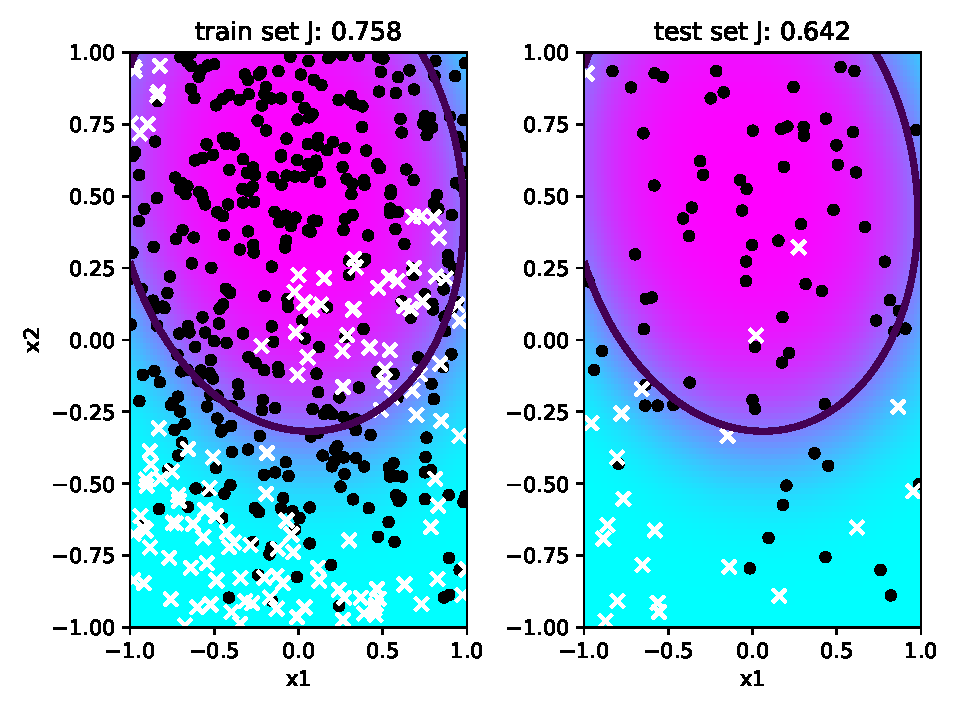
\includegraphics[width=\textwidth]{./Figures/logreg3_eta20_decbound.pdf}
\caption{Decision boundary, $\eta=20$}
\end{subfigure}
}
\caption{GD errors and decision boundaries for varying learning rate $\eta$, degree $l=2$ and 200 iterations.}
\label{logreg3}
\end{figure}

\begin{figure}[!ht]
\vspace*{-53.6pt}
\centering
\makebox[\textwidth]{
\begin{subfigure}{0.5\textwidth}
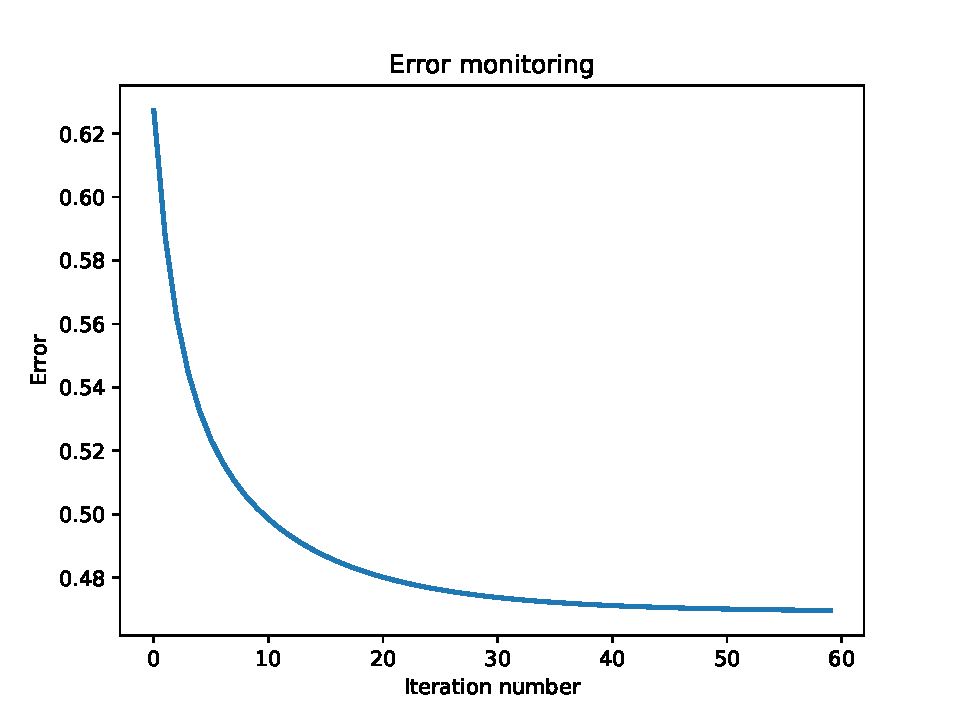
\includegraphics[width=\textwidth]{./Figures/logreg4_deg1_opt_error.pdf}
\caption{Error, $l=1$, $\eta=1$, 60 iterations}
\end{subfigure}
\begin{subfigure}{0.5\textwidth}
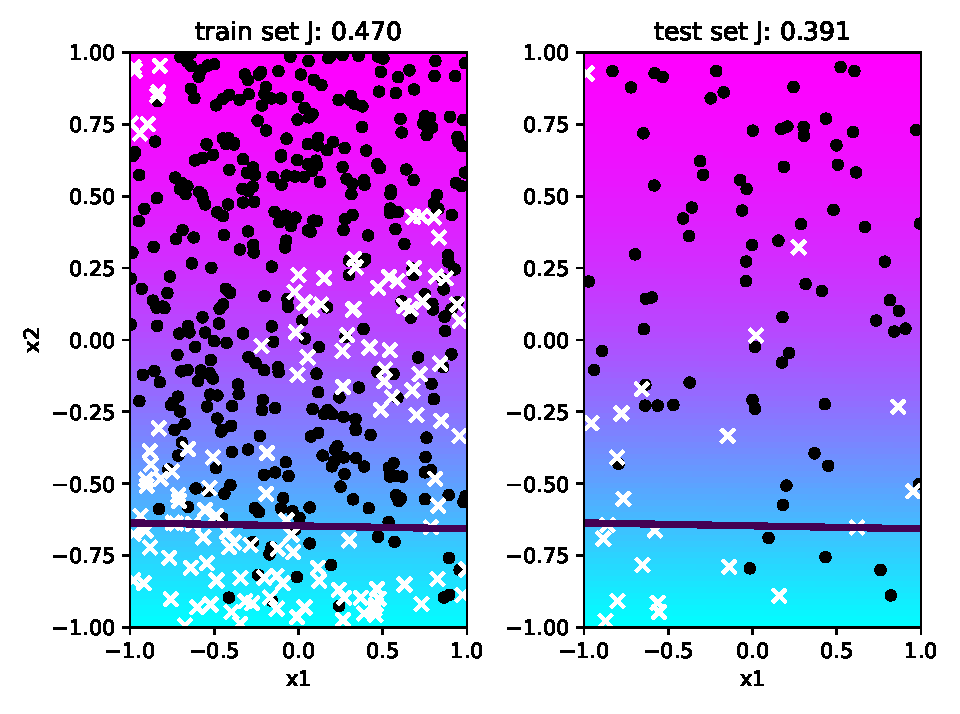
\includegraphics[width=\textwidth]{./Figures/logreg4_deg1_opt_decbound.pdf}
\caption{Decision boundary, $l=1$, $\eta=1$, 60 iterations}
\end{subfigure}
}

\makebox[\textwidth]{
\begin{subfigure}{0.5\textwidth}
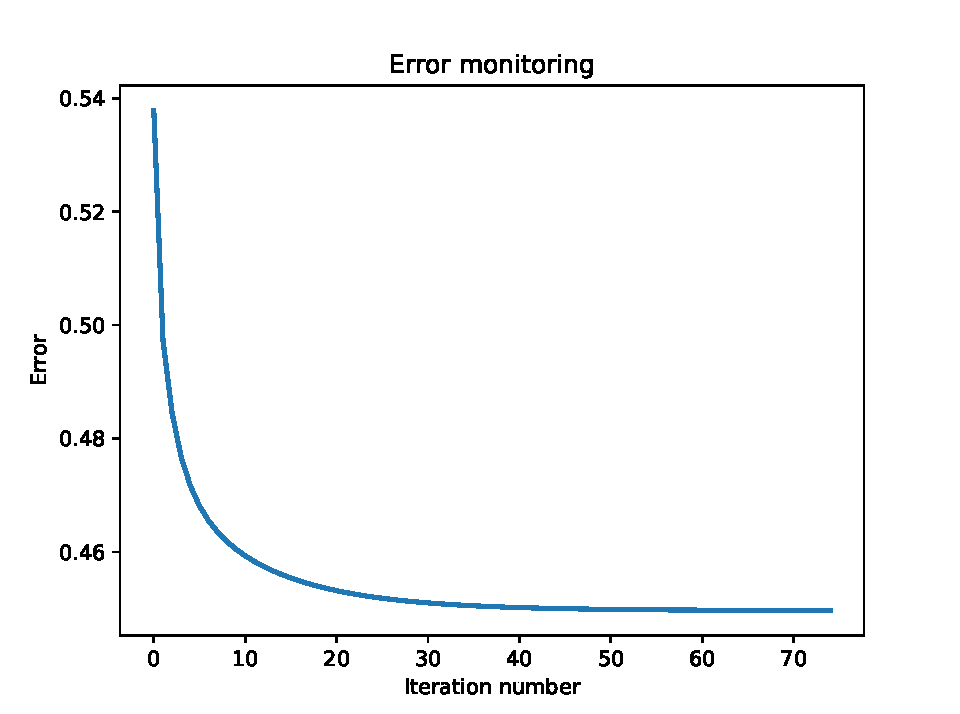
\includegraphics[width=\textwidth]{./Figures/logreg4_deg2_opt_error.pdf}
\caption{Error, $l=2$, $\eta=5$, 75 iterations}
\end{subfigure}
\begin{subfigure}{0.5\textwidth}
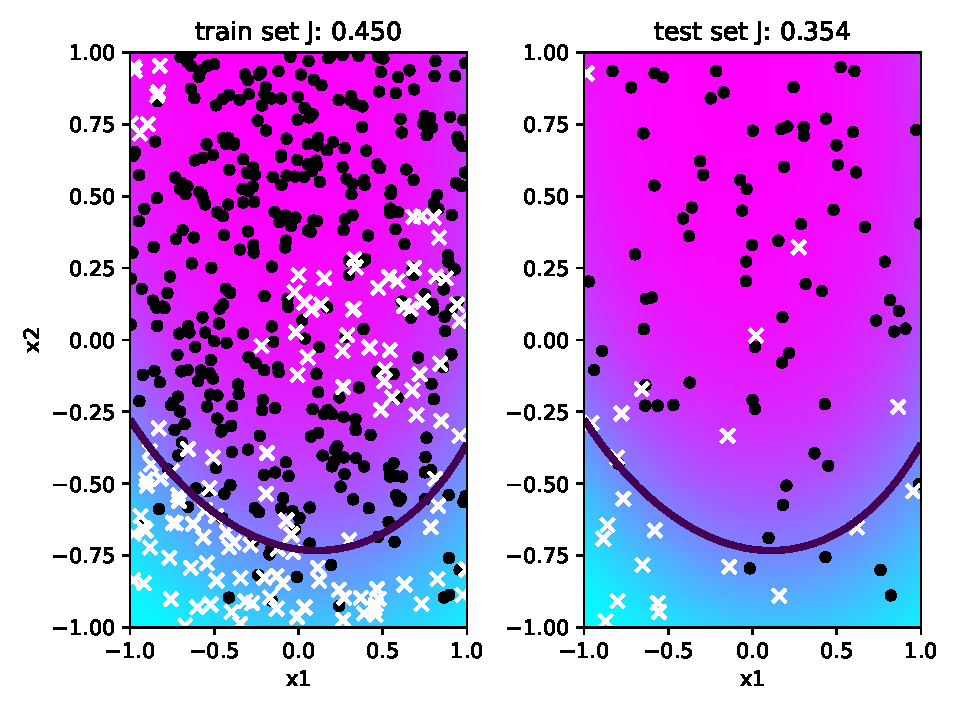
\includegraphics[width=\textwidth]{./Figures/logreg4_deg2_opt_decbound.pdf}
\caption{Decision boundary, $l=2$, $\eta=5$, 75 iterations}
\end{subfigure}
}

\makebox[\textwidth]{
\begin{subfigure}{0.5\textwidth}
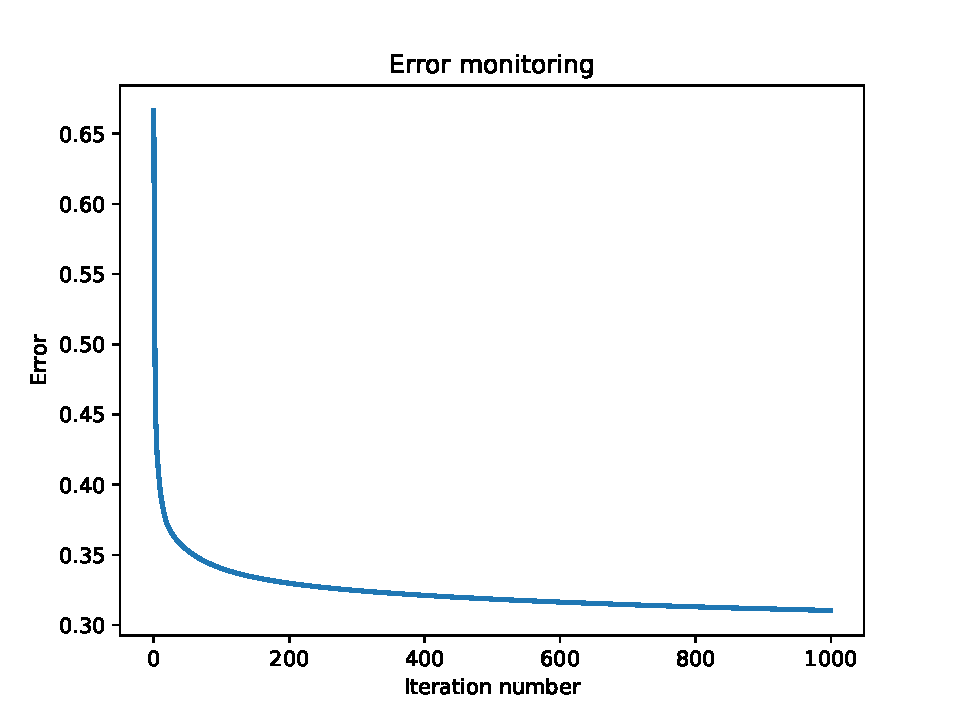
\includegraphics[width=\textwidth]{./Figures/logreg4_deg7_opt_error.pdf}
\caption{Error, $l=7$, $\eta=10$, 1000 iterations}
\end{subfigure}
\begin{subfigure}{0.5\textwidth}
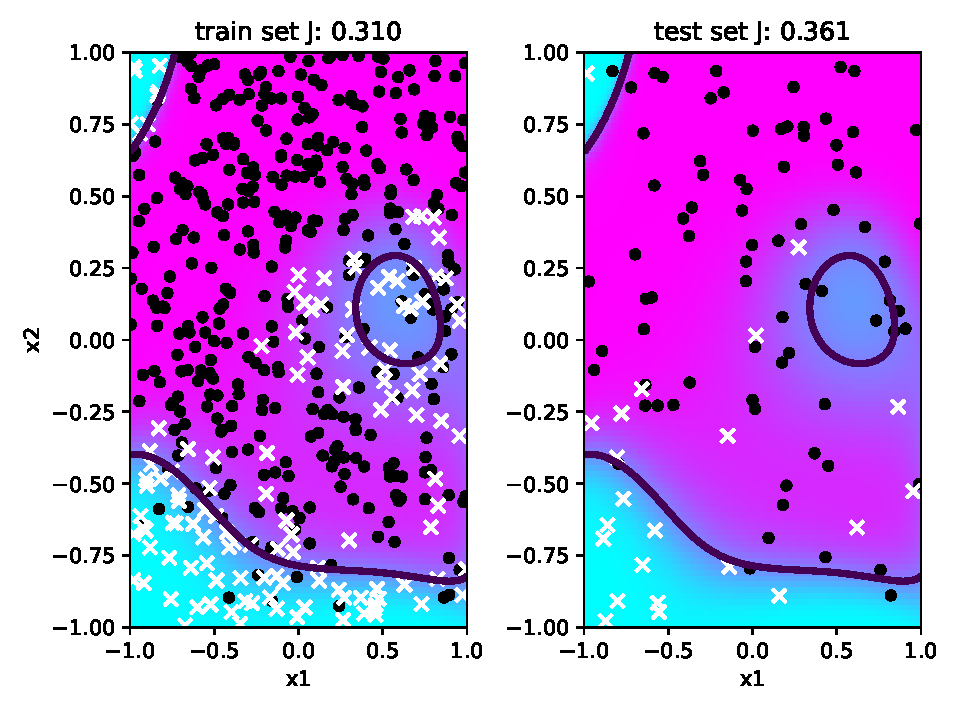
\includegraphics[width=\textwidth]{./Figures/logreg4_deg7_opt_decbound.pdf}
\caption{Decision boundary, $l=7$, $\eta=10$, 1000 iterations}
\end{subfigure}
}

\makebox[\textwidth]{
\begin{subfigure}{0.5\textwidth}
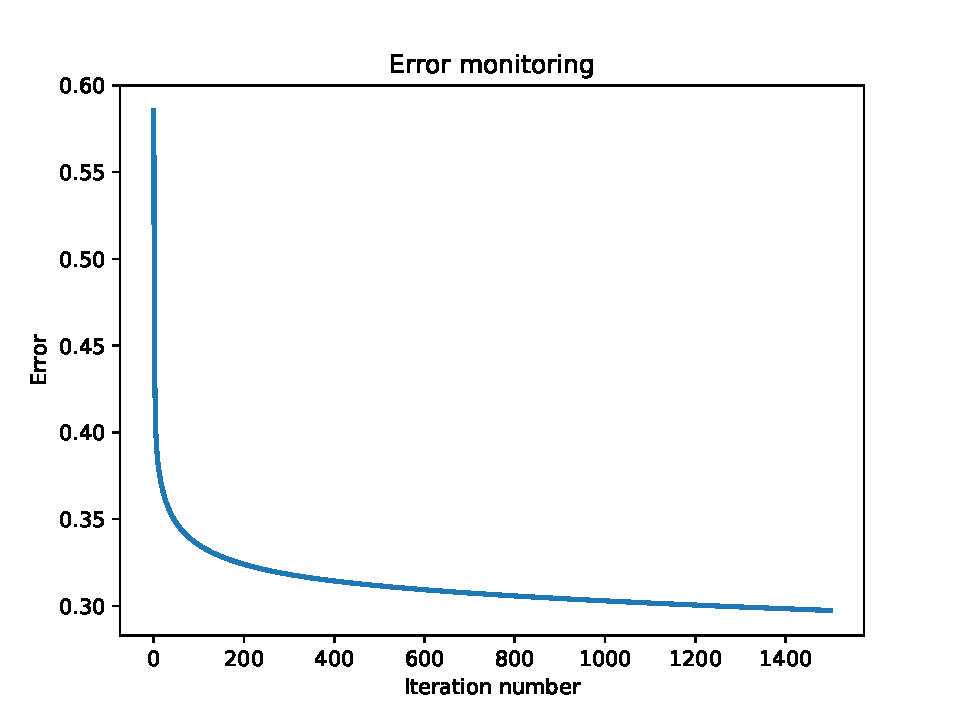
\includegraphics[width=\textwidth]{./Figures/logreg4_deg20_opt_error.pdf}
\caption{Error, $l=20$, $\eta=8$, 1500 iterations}
\end{subfigure}
\begin{subfigure}{0.5\textwidth}
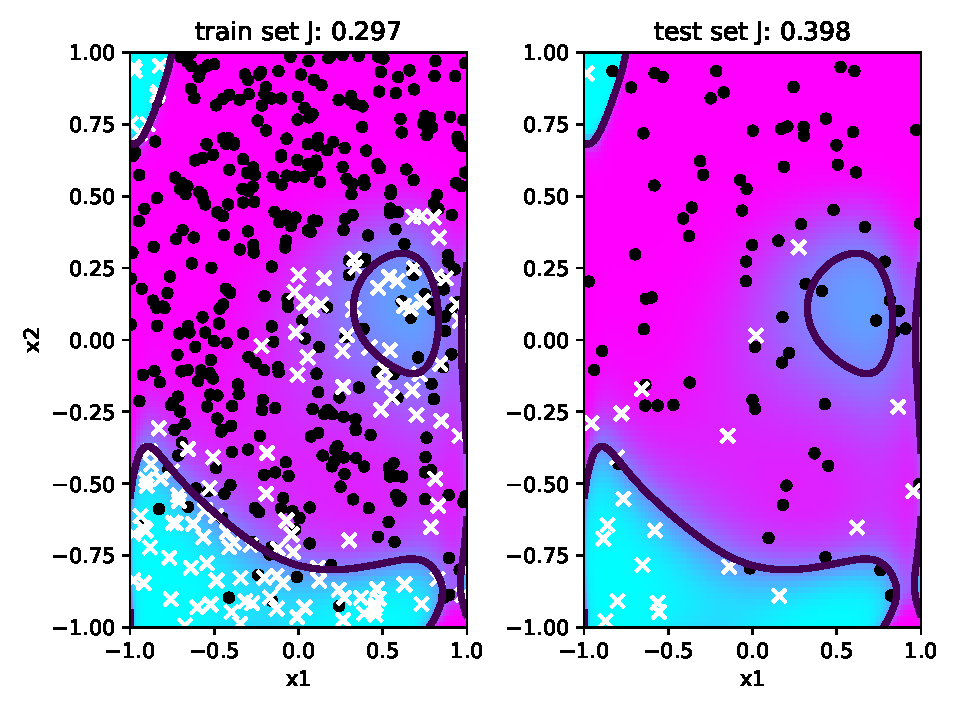
\includegraphics[width=\textwidth]{./Figures/logreg4_deg20_opt_decbound.pdf}
\caption{Decision boundary, $l=20$, $\eta=8$, 1500 iterations}
\end{subfigure}
}
\caption{GD errors and decision boundaries for degrees $l=1,2,7,20$ and chosen parameter values.}
\label{logreg4_fig}
\end{figure}

\begin{table}[!ht]
\centering
\begin{tabular}{|c||c|c||c|c|}
\hline
degree $l$ & learning rate $\eta$ & iterations & training cost & testing cost \\ \hline \hline
1          & 1                    & 60         & 0.470         & 0.391        \\ \hline
2          & 5                    & 75         & 0.450         & 0.354        \\ \hline
7          & 10                   & 1000       & 0.310         & 0.361        \\ \hline
20         & 8                    & 1500       & 0.297         & 0.398        \\ \hline
\end{tabular}
\caption{Chosen values for learning rate $\eta$ and number of iterations and obtained training and testing costs for degrees $l=1,2,7,20$.}
\label{logreg4_tab}
\end{table}


\end{document}}